%---------------------------------------------------------------------------%
%->> Main content
%---------------------------------------------------------------------------%
\section{选题的目的和意义}
代码摘要(code summary)也称为代码注释(code comment),是对一段源代码简短的自然语言描述,其目的是让人们能够更加轻松地了解代码。注释是编写程序时,写程序的人给一个语句、程序段、函数等的解释或提示,能提高程序代码的可读性。代码自动摘要技术(code summarization)通过自动化地生成代码摘要辅助开发者更好地理解程序代码,该技术在许多软件开发活动中都具有重要的应用价值\cite{zsk}。

\subsection{选题背景与目的}
随着软件代码规模的日益增长,程序员所面临的代码开发和维护压力越来越大。如何辅助开发人员理解代码,以提高软件开发的效率和质量,已成为软件工程领域的研究热点\cite{yqf}\cite{hx}。

据统计,在软件开发生命周期中,近90\%的工作是维护,其中大部分工作是用在理解维护任务和相关源代码\cite{nosek1990software}。在代码复用和软件维护过程中,对程序的理解是代码修改的先决条件。代码注释作为源代码的自然语言描述,总结了代码背后的思路,能够帮助开发人员快速理解代码的。新手在学习一门新的开发语言时也可以通过阅读注释加快学习过程。然而在实际开发过程中,程序员不断地为代码编写和更新注释效率低且准确度难以保证,面临着注释易丢失、易过时的问题,缺乏注释和过时的注释都会降低软件项目的可维护性和可用性。为了解决注释不足的问题,研究人员作出了很多尝试,例如使用描述性的标志符名称问,然而完整描述代码功能的标志符会导致很长的标志符名称,较长的名称反而会降低代码的可读性\cite{binkley2008impact}。诸如JavaDoc和Doxygen之类的工具可以自动将注释的格式文档化,但仍然依赖于开发人员编写文本和示例,且很多软件都缺乏能够描述软件功能的文档\cite{lwp}。通过模型自动生成代码的注释不仅能节省开发人员编写注释的时间,同时有助于理解代码。因此,自动化注释生成是软件工程领域一个重要而富有挑战性的研究方向\cite{jz}。

\subsection{选题意义}
代码注释自动生成涉及到自然语言和程序语言的联合处理,相关研究还有从自然语言描述自动生成代码和通过自然语言查询进行代码搜索 \cite{lx} 等任务。将注释自动生成与程序自动生成相融合,可以减轻程序员的开发负担,实现开发效率和质量的提高,对提高软件开发的自动化程度具有重要意义;将注释自动生成与代码搜索相结合,以代码注释作为搜索的索引,可以更符合人的搜索习惯,既可以增强程序理解,又能提升代码搜索的效果。除此之外,如今的开源社区和开源代码网站(如StackOverflow和GitHub)上的海量代码资源没有注释,利用注释自动生成技术为这些无注释的代码补充注释,丰富代码资源库,从而使这些代码资源所蕴涵的众多知识和群体智慧被充分利用,将为软件开发工作提供很大的帮助。这些任务可以提高程序员的生产力,因此具有很大的实际意义;而且由于它们的困难以及自然语言、计算和推理之间的推测联系,它们也具有科学意义\cite{miceli2017parallel}。


\section{与本课题相关的国内外研究现状}
研究人员可以从多个角度为源代码添加注释。自动源代码注释工具正在成为不需要人工干预就可以生成注释的可行技术。这些技术大致可分为如下几种方法:基于规则、基于自动文本摘要、基于数据、基于主题模型、基于深度学习,各个方法年代分布如图\ref{fig: fig1}所示。

通过近年来分布情况可以看出,超过60\%的论文在2015年之后发表,近50\%的论文发表于2016年之后。最早使用的是基于规则的方法,随着神经网络的发展,基于深度学习的注释生成方法在 2015 年出现并逐年增多,最近的研究主要使用的是深度学习的技术。

\begin{figure}
	\centering
	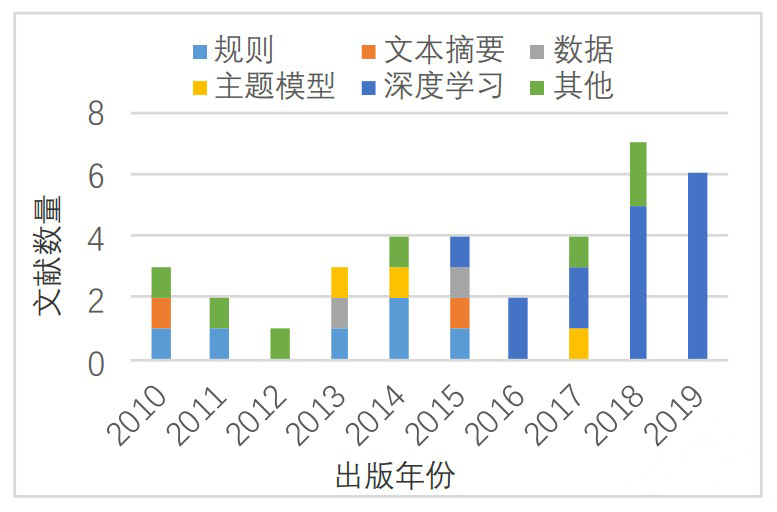
\includegraphics[width=0.6\textwidth]{1.jpg}
	\caption{文献年代分布}
	\label{fig: fig1}
\end{figure}

\subsection{早期方法}
早期代码摘要方法大致可分为基于规则的方法、基于文本摘要的方法、基于数据驱动的方法及基于主题模型的方法。

基于规则的方法通过选择与源代码结构密切相关的详细信息,然后制定规则使其与给定源代码紧密匹配以生成准确的注释。Sridhara定义启发式规则为Java方法生成注释\cite{sridhara2010towards}。Moreno L等人关注代码的结构信息,基于文本生成工具和启发式规则为Java类生成注释\cite{moreno2013automatic},实验为两个系统生成了40条注释,准确率达到96\%,但是该方法生成注释产量较低。McBurney 等人认为方法的上下文信息有助于理解方法存在的原因以及它在软件中所起的作用,使用SWUM(software word usage model,软件用词模型)提取方法的关键字\cite{mcburney2014automatic},用自然语言生成系统生成描述方法上下文信息的注释,该方法表明包含代码上下文信息的注释更受程序员欢迎。

基于自动文本摘要的方法首先通过信息检索抽取出代码中最重要的信息,从源代码中抽取词汇信息(如标志符、注释等)并将其预处理,去除停用词 (stopwords) 和编程语言关键字,将标志符拆分成单词,并使用词干替代。将代码转换为文本的语料库,然后使用文本的信息检索(IR)方法确定文本的若干个术语单词,结合代码的结构信息构成摘要性注释。Haiduc等人提出了代码摘要的概念\cite{haiduc2010use},略读代码和阅读代码都过于极端,略读虽快但会导致误解,而细读代码又很耗时。王金水等人基于句法分析技术 (syntactic analysis),利用词性标注识别出代码中的名词集合,然后通过块分析修正词性标注阶段可能引入的错误,在降噪之后再从中选取若干个权值最高的词以生成代码摘要\cite{wjs}。

随着开源社区的发展,研究人员可以获取大量高质量的代码资源,其中包含着许多信息可被应用于软件开发中。Wong 等人从问答网站 (StackOverflow) 上挖掘问答数据,获取代码及其对应的自然语言描述,与相似的代码片段进行匹配,将其改进处理后可作为新代码片段的注释\cite{wong2013autocomment}。

主题模型 (topic models) 是一种统计模型,其中单词与其他单词之间的关联取决于它们在文档中的共现比例。文献\cite{mcburney2014improving}使用主题模型选择关键字和主题作为源代码摘要,结果有 76.9\%的注释符合评估标准。李文鹏等人基于LDA (latent dirichlet allocation) 主题模型,挖掘软件文档中的系统功能描述,从源代码中提取主题并结合 LexRank 算法生成简短摘要\cite{lwp}。


\subsection{基于深度学习的方法}
深度学习是一种数据驱动的端到端的方法,根据已有数据构建神经网络对数据中隐含的特征进行挖掘,已在众多领域中成功应用。在代码注释自动生成任务中,运用深度学习技术自动地学习程序代码中蕴涵的特征,可取代传统方法中繁琐的人工特征提取过程,这种方法在如今大数据时代具有巨大的优势:避免了人工设计特征的误判,数据量越大,深度学习得到的分布表示结果越好。常用的深度学习技术包括卷积神经网络 (convolutional neural network,CNN)、循环神经网络(recurrent neural network,RNN)和其变体长短时记忆(long short-term memory,LSTM)网络、门控循环单元(gated recurrent unit,GRU)、注意力机制(attention)等。

Allamanis 等人应用基于注意机制的CNN 学习代码的长期特征和本地信息,从GitHub获取了11个Java项目构造代码-注释数据集\footnote{\url{groups.inf.ed.ac.uk/cup/codeattention}},为 Java 方法生成注释\cite{allamanis2016convolutional}。Moore等人提出了与语言无关的注释生成方法,将 CNN 和 LSTM 组合构建模型,获取字符信息,基于MUSE语料库\footnote{\url{http://muse-portal.net/}}创建了Java、C++和Python的代码-注释语料库\cite{moore2019convolutional}。相较于 CNN,RNN 能够记忆更长的代码序列信息。Iyer等人采用 RNN 将代码作为纯文本处理,利用注意机制将注释中的单词与代码标记进行对齐,提出CodeNN\cite{iyer2016summarizing}\footnote{\url{https://github.com/ sriniiyer/codenn}}。Leclair 等人利用两个 GRU 层将代码的AST 信息和单词信息进行编码,通过注意机制将单词和 AST的向量连接起来以创建上下文向量,然后生成代码的摘要\cite{leclair2019neural}。Hu等人提出了含有两个编码器的模型(API编码器和代码编码器),RNN解码器利用所学的API知识,将两个编码器的信息进行整合\cite{hu2018summarizing}。该模型的性能与不含 API信息的模型相比,在 BLEU-4 得分上提高了 41.98\%。可见,代码的 API 调用中包含了代码功能的重要信息,有助于提高注释生成的准确率。Wan 等人使用强化学习缓解了 exposure bias 问题,利用一个LSTM表示代码的序列信息,另一个基于AST的LSTM表示代码的结构信息,将两种信息结合生成代码注释\cite{wan2018improving}。该方法在多个自动评估指标上取得了不错的分数,到目前为止,基于强化学习的代码注释生成研究较少,所以这是一个值得研究的方向。

大多数基于AI (人工智能) 的代码摘要任务的灵感都来源于自然语言处理领域中的神经机器翻译 (neural machine translation,NMT),NMT 通常基于seq2seq将一种自然语言转换为另一种自然语言\cite{leclair2019neural}。Hu 等人使用机器翻译模型来解决源代码摘要任务\cite{hu2018deep}。为了保留代码中的结构信息,提出了一种新的遍历方法(SBT),遍历代码的 AST并转换成线性序列,该模型比基于 token 序列的模型性能提高了约 10\%。Zheng 等人基于注意力机制利用代码的结构信息提取功能语义,例如关键语句、符号和关键字等,通过将代码中的标志符和符号分开处理,该模型能以更结构化的方式理解代码\cite{zheng2019codeattention}。


\section{课题研究的可行性分析}
代码自动摘要经过近十年的发展,已经形成了独立的分支并拥有扎实的理论基础和合理的研究方法。自2010年起,软件工程和人工智能领域的期刊和国际顶级会议如 FSE、ASE、ICSE、ICPC、EMSE等都持续有该领域文章发表,且数量逐年增多。前文所述基于神经网络、注意机制以及大量数据的输入在注释生成任务上取得了较好的效果。

同时,关于该领域的研究拥有大量的数据集作为支撑。运用深度学习技术自动地学习程序代码中蕴涵的特征,可取代传统方法中繁琐的人工特征提取过程,这种方法在如今大数据时代具有巨大的优势:避免了人工设计特征的误判,数据量越大,深度学习得到的分布表示结果越好。作为软件工程领域研究的重要内容之一,代码注释自动生成正在随着各项技术的发展不断推进,展示了极具竞争力的性能和广阔的发展前景。在未来,随着人工智能与深度学习技术的发展,互联网中涌现出的大量可利用代码及注释资源为研究者们提供了利用大规模注释中包含的知识来完成注释生成任务的新途径。本文从注释生成的相关概念出发,对现有代码注释自动生成技术进行了介绍与分析,讨论了注释自动生成的相关应用,在此基础上揭示了代码注释自动生成技术有待解决的挑战,以期为相关的研究者和工程技术人员提供一定的参考。


\section{课题研究的策略、方法和步骤}
课题研究的策略为:通过文献研究法分类阅读有关文献(包括文字、图形、符号、声频、视频等具有一定历史价值、理论价值和资料价值的材料)记录新颖独特的观点,有价值的意见、方法。发现问题、分析问题、提出假设、验证假设。进而搜集材料、分析、归纳、提出观点、整理提炼、分析总结。

课题研究方法和步骤遵循主流的代码摘要方法,其一般框架可分为注释复用及注释抽取:注释复用技术是从已有的代码片段中匹配将要被注释的代码并获取其中的注释,利用优化技术将原有注释处理后输出为目标注释;注释抽取技术通过提取代码的结构及语义信息,对其进行预处理,然后构建注释生成模型,利用自然语言处理技术结合程序的语法结构将这些单词组合成为陈述语句并输出为代码注释。本文所使用的方法属于注释抽取。



\section{预期成果形式描述}
论文


%\nocite{*}% 使文献列表显示所有参考文献(包括未引用文献)
%---------------------------------------------------------------------------%
